\section{Sequence Modeling} \label{sec:background-sequence-modeling} 

Machine learning systems face many problems where they must consider a sequence of inputs on one or more sensory channels. That is, their predictive model is dependent on a sequence of data points. For example, an autonomous vehicle that learns to move by analyzing sequences of frames from a video, depends on previous frames in the input sequence to infer context. It is therefore important to extend the traditional neural network models to consider temporal information as well as spatial information\cite{DBLP:journals/corr/Lipton15}.

One approach to this type of problem is to explicitly capture sequential information or context by concatenating the inputs by a specific number of its predecessors or successors. This effectively creates a sliding window that scans the sequential data\cite{DBLP:journals/corr/Lipton15}. An example of this approach is seen in the work done by Mikolov et al. 2013 where the dimensionality of a corpus of text represented using the bag of words technique (words from a corpus are represented using a sparse vector where each feature of the vector corresponds to a word and the occurrence of a specific word is expressed by setting the word's corresponding feature in the vector) is considerably reduced to a much smaller vector and at the same time maintaining context between words such that words that often appear in the same context would have vectors in close proximity to one another\cite{DBLP:journals/corr/abs-1301-3781}. The drawback to this approach however is that the length of the sequence is fixed and therefore the effect of time on the inputs is limited to some extent.

Certain applications rely on having the ability to model arbitrarily long sequences of inputs. In this section we introduce a type of neural network models called recurrent neural networks (RNNs). This type of architecture allows some inputs to be represented as a function of previous outputs and can learn how much influence these previous outputs can have on the current output\cite{DBLP:journals/corr/Lipton15}. We also introduce a variation of RNNs that overcome a major limitation known as the vanishing gradient problem.

\subsection{Recurrent Neural Networks} \label{sec:background-sequence-modeling-recurrent-neural-networks}

\begin{figure}[t]
	\centering
	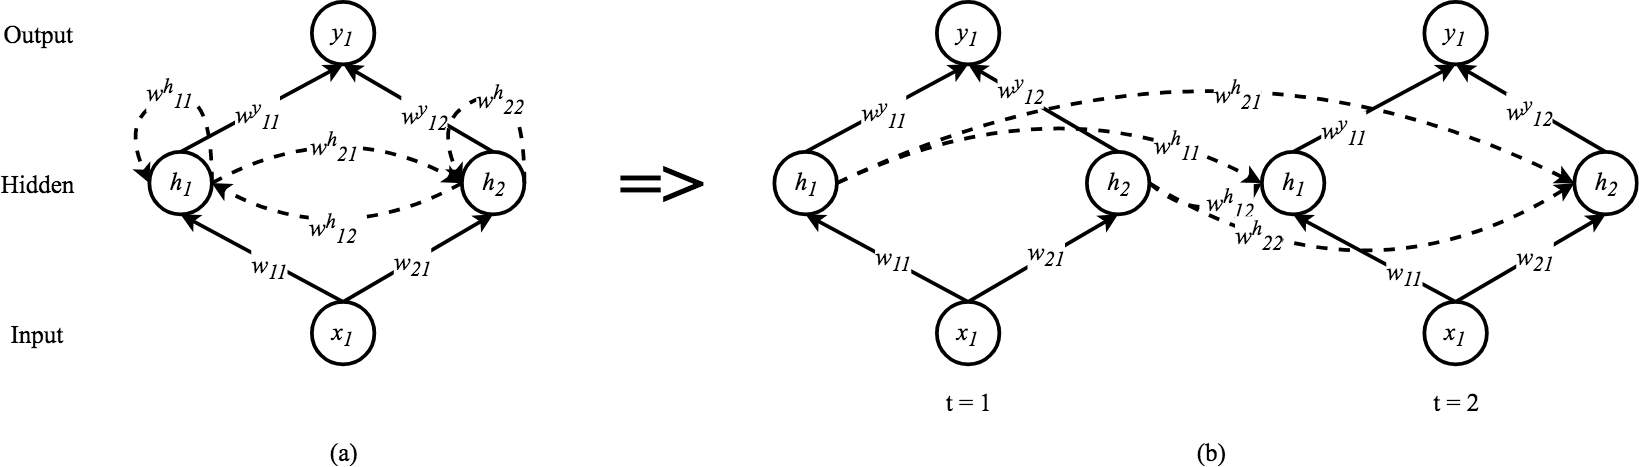
\includegraphics[max width=\textwidth]{recurrent-neural-network}
	\caption{A recurrent neural network with one hidden layer consisting of two units (a). The same neural network in (a) that is unfolded into two time steps (b)\cite{DBLP:journals/corr/Lipton15}.}
	\label{fig:recurrent-neural-network}
\end{figure}

A recurrent neural network is a feed forward neural network with additional connections between the nodes in one or more hidden layers called recurrent connections. These recurrent connections, connect the weighted output of each hidden node to another hidden node across a single time step. It is important to note that these recurrent connections do not form cycles within a single time step. The weights carried by these recurrent edges represent state that is remembered from one time step to the next and it is through this state that the recurrent neural network learns to infer context\cite{DBLP:journals/corr/Lipton15}.

Figure \ref{fig:recurrent-neural-network} (a) shows a recurrent neural network with one input unit, one output unit and a hidden layer with two units. It also shows the recurrent connections in the hidden layer. Each node in the hidden layer receives inputs from the data point $x$ and from each hidden unit $h$ in the previous time step. Figure \ref{fig:recurrent-neural-network} (b) shows the same recurrent neural network that is unfolded into two time steps. Notice that the recurrent connections are no longer depicted as cyclic connections.

Unfolding the recurrent neural network into its component time steps allows us to identify the formula used to calculate the output of each hidden node:
\begin{equation}
	h_{h}^{(t)} = \sigma(W_{hx} x^{(t)} + W_{hh} h^{(t - 1)} + b_{h})
\end{equation}
Where $W_{hx}$ is the weight matrix from the input at the current time step to the hidden unit $h$, $ x^{(t)}$ is input at the current time step, $W_{hh}$ is the weight matrix from the hidden unit $h$ at the previous time step to the same hidden unit at the current time step, $ h^{(t - 1)}$ is the output of the hidden unit $h$ from the previous time step and finally, $b_{h}$ is the bias for the hidden unit $h$\cite{DBLP:journals/corr/Lipton15}.

Unfolding recurrent neural networks also helps us visualize them as deep architectures. Each time step can be considered a layer in a deep neural network. This allows us to use the backpropagation algorithm to train recurrent neural networks using a variation known as backpropagation through time (BPTT)\cite{DBLP:journals/corr/Lipton15}.

\subsection{Long Short-Term Memory Units} \label{sec:background-sequential-models-long-short-term-memory-units}

\begin{figure}[t]
	\centering
	\includegraphics[max width=\textwidth]{lstm-gates}
	\caption{Internal architecture of a Long Short-Term Memory unit showing the three gates and the flow of input, output and cell state\cite{LSTM}.}
	\label{fig:memory-cell}
\end{figure}

The previous section showed how recurrent neural networks can be trained by unfolding the network into a multi-layer feedforward network in a process called backpropagation through time. The problem with BPTT is the same as with deep neural networks, the backward propagation gradient can become very small. For example, if the hidden layers use the hyperbolic tangent activation function, given that the gradient of this function falls in the interval $[0, 1]$, multiplying such small numbers $n$ times for $n$ layers will result in an update rule that makes exponentially smaller changes as $n$ increases. An architecture that is significantly deep, or in the case of RNNs contains many time steps, will have an update rule that makes little or no change to the weights of the lower layers of the network\cite{Bengio:1994:LLD:2325857.2328340}. This problem is known as the vanishing gradient. Because of the vanishing gradient problem, standard RNNs are unable to model sequences that are arbitrarily long. In 1997, Hochreiter and Schmidhuber introduced a new type of RNN architecture that used Long Short-Term Memory (LSTM) units.\cite{hochreiter1997long}. 

LSTM units, such as the one shown in Figure \ref{fig:memory-cell}, replace the traditional hidden layer units found in recurrent and feedforward networks, like those with $tanh$ activation functions. LSTM layers introduce a connection between adjacent time steps called the constant error carousel (CEC). The CEC constrains the vanishing gradient by fixing the weights on this connection to 1. The value carried by the CEC from one time step to the next is called the cell state ($C_t$). The cell state acts as the memory of the LSTM network that remembers relevant information from previous inputs and influences the output on subsequent time steps. This is made possible due to the presence of three gating structures that control the flow of information on the cell state. A gate, as shown in Figure \ref{fig:memory-cell}, is a sigmoid unit with its own set of weights, the output of which is multiplied by the current cell state. The output of the sigmoid unit is a value in the range of 0 to 1, where 0 indicates that no information is retained and 1 indicates that everything is kept\cite{LSTM}. The following explains the role of each gate structure in more detail.

\subsubsection{Forget Gate}

The forget gate decides how much information on the cell state needs to be forgotten based on the output from the previous time step and the current input. It's a sigmoid gate that outputs a value, $f_t$, in the interval $[0, 1]$, where 0 means nothing is retained while a 1 means everything is retained\cite{LSTM}. The following is the formula for the forget gate output:
\begin{equation}
f_t = \sigma(W_f[h_{t-1}, x_t] + b_f)
\end{equation}

\subsubsection{Input Gate}

The input gate determines how much of the input contributes to the cell state at this point in the sequence. It updates the cell state in two steps. First, a sigmoid unit determines a value, $i_t$, in the interval $[0, 1]$, that controls how much information from a vector $\hat{C}_t$ of potential values is added to the cell state. $\hat{C}_t$ is generated in the second step by running the input $x_t$ into a $tanh$ unit. Finally, the output from this gate is combined with the output from the forget gate to determine the value of the cell state at the current time step\cite{LSTM}.
\begin{equation}
i_t = \sigma(W_i[h_{t-1}, x_t] + b_i)
\end{equation}
\begin{equation}
\hat{C}_t = tanh(W_C[h_{t-1}, x_t] + b_C)
\end{equation}
\begin{equation}
C_t = f_t * C_{t-1} + i_t * \hat{C}_t
\end{equation}

\subsubsection{Output Gate}

Finally, the output gate determines how much of the internal state influences the output at the current time step. Like the forget gate, the output gate generates the output $h_t$ in two steps. First, a sigmoid unit determines a value, $o_t$, in the interval $[0, 1]$, that controls how much of the state goes to the output. The internal state is then scaled to the range $[-1, 1]$ using a $tanh$ function and then combined with the value of the output gate to determine the output\cite{LSTM}.
\begin{equation}
o_t = \sigma(W_o[h_{t-1}, x_t] + b_o)
\end{equation}
\begin{equation}
h_t = o_t * tanh(C_t)
\end{equation}